% !TEX root = mainthesis.tex

%Chapter 4


\renewcommand{\thechapter}{4}


\chapter{Making BECs in the Rubidium Lithium apparatus}

All the experiments presented in this thesis were performed at the Rubidium-Lithium (RbLi) apparatus at the University of Maryland. The experiment was designed to produce mixtures of quantum degenerate gases of bosons and fermions. The original plan was abandoned because the cross-species scattering length was found to be repulsive and small ($a_s\approx20\,a_B)$~\cite{silber_quantum-degenerate_2005} and the nearest heteronuclear $s$-wave Feshbach resonance was measured to occur at the unexpectedly large magnetic field of $\unit[1066]{G}$~\cite{deh_feshbach_2008} and therefore all our experiments were performed using only $\Rb87$.

As of the time this thesis is being written, the apparatus is scheduled to be shut down and the construction of a new dual-species apparatus for $\Rb87$ and K$^{39}$ is underway. I will not describe in detail the technical details of the RbLi apparatus which have been extensively discussed in the theses of former lab members~\cite{CampbellThesis,PriceThesis}. Instead I will focus on describing elements of the experiment that either worked exceptionally well or exceptionally poorly, some sort of `to-do' and `not-todo' list. Additionally in Appendix~\ref{app:Basement_lab} I will describe technical aspects of the construction of the new apparatus where I was involved. 


\section{The RbLi vacuum system}

The RbLi vacuum system has a dual species oven designed for both Rb and Li. Both Rb and Li atoms are heated up. The Rb oven was kept at $\unit[120]{C}$ while the Li oven at $\unit[160]{C}$, below the temperature required to make an atomic beam. The heated atoms traveled to the main oven chamber that is pictured in Figure~\ref{fig:RbLi}b containing a cold-cup and an oven shutter. The cold-cup is a cylindrical shaped copper piece that is attached to the cold end of a thermo-electric cooler (TEC) via a copper rod. We kept the cold-cup temperature at $-\unit[30]{C}$ in order to capture excess Rb atoms in the chamber and prevent damaging the ion pumps.
On January 2018 we noticed that an excessive buildup of Rb atoms in the cold cup was blocking the atomic beam. To remedy this issue we closed the gate valve between the oven and the Zeeman slower to make sure the UHV portion stayed clean. We then reversed the polarity of the TEC that provides the cooling of the cold cup and we heated the TEC just enough to see the Rb atoms melt and clear path of the atomic beam. Finally we cooled the TEC back to $\unit[-30]{C}$ and waited a full day before opening back the gate valve. 

\begin{figure*}[htb]
\begin{center}
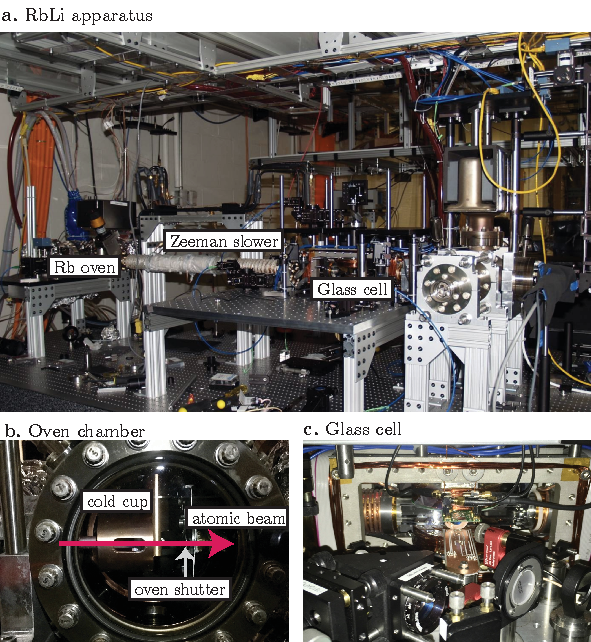
\includegraphics[]{Figures/Chapter4/RbLi.pdf}
\caption[$\Rb87$ level structure]{$\Rb87$ level structure (not to scale). {\bf a.} Ground and first excited state electronic configuration of $\Rb87$ given by the $\{n,\mathbf{L}\}$ quantum numbers. {\bf b.} The interaction between the orbital angular momentum and the spin of the electron leads to the fine splitting of orbitals with $L>0$. The splitting of the $5^2P$ line gives rise to the D1 and D2 lines. {\bf c.} The interaction between the total angular momentum and the nuclear spin causes the fine structure levels to split further into states characterized by the quantum number $F$.}
\label{fig:RbLi}
\end{center}
\end{figure*}

The oven shutter allowed us to block or enable the atomic beam. We used a home made device, made from a repurposed hard drive disk shutter with a metalic flag attached to its end. The shutter was electrically connected to en electric feedthrough with vacuum-compatible Kapton sealed wires. We never experienced any troubles with our shutter, unlike one other apparatus~\cite{BrownThesis} within the JQI which used a \noted{Uniblitz} commercial shutter that failed and had to be replaced. The home made vacuum shutter is the first element in the `to-do' list.  

From the oven chamber the atomic beam travels down a Zeeman slower~\cite{phillips_laser_1982 } (see Figure~\ref{fig:RbLi}) where atoms were laser cooled. The Zeeman slower additionally acts as a differential pumping stage between the oven side and the ultra-high vacuum (UHV) side. The UHV side has a glass cell (Figure~\ref{fig:RbLi}a,c) where the atoms are trapped and further cooling is performed to achieve Bose-Einstein condensation. 

\subsection{Magnetic field control}


Technical things worth talking about:

-fiber splitter
-dipole trap and fiber couopling with mode expanders
-use of non-pm fibers with paddles
-water cooling system (including interlock of the Zeeman slower?)
-High power RF antenna stuff
-Oven shutter
-Microwaves and stub tunning
-Mako camera
-Labscript



\section{Laser systems}
\subsection{Master and cooling laser systems}
\subsection{1064nm laser system}
\subsection{Raman laser system}
\subsubsection{Tapered amplifier laser system}
\subsubsection{Ti:Saphire and 532 nm laser system}

\section{Imaging systems}
\subsection{The xy imaging system}
\subsection{The zx imaging system}
\subsection{Measuring magnification and focus?}

\section{Water cooling}

\section{Magnetic field control}
\subsection{Bias coils}
\subsection{Gradient cancelation coils}

\section{RF electronics}
\subsection{RF evaporation antenna}
\subsection{High power RF antenna}
\label{sec:high_power_rf_antenna}
The antenna loop is Digikey part number $732-5646-ND$

\section{Microwave electronics}

\section{Computer control and data acquisition}
Cite labscript. 
\section{Experimental sequence to make BECs}
\label{sec:making-becs}



\section{Quantum coherent dynamics}
\label{sec:quantum_coherent_dynamics}

\subsection{The Rabi cycle}
\label{seq:rf_coupling}
RF coupling and microwave coupling
\subsection{Ramsey interferometer}
\note{TODO:include Ramsey fringes from synthetic clock states}
\subsection{Adiabatic rapid pasage}
\label{sec:arp}

\subsection{Ramsey interferometry}
\subsection{Partial transfer absorption imaging: magnetic field stabilization}
\label{sec:ptai}
We then apply a pair of $250\,\mu\mathrm{s}$ microwave  pulses that each transfer a small fraction of atoms into the $5^2{\rm S}_{1/2}$ $f=2$ manifold that we use to monitor and stabilize the bias field \cite{leblanc_direct_2013}. The microwave pulses are detuned by $\pm 2\, \kHz$ from the $\ket{f=1,m_F=0}\leftrightarrow\ket{f=2,m_F=1}$ transition and spaced in time by $33\, \mathrm{ms}$ (two periods of $60\, \mathrm{Hz}$). We imaged the transferred atoms following each pulse using absorption imaging\footnote{We did not apply repump light during this imaging, so the untransferred atoms in the $f=1$ manifold were largely undisturbed by the imaging process.}, and count the total number of atoms $n_1$ and $n_2$ transferred by each pulse. The imbalance in these atom numbers $(n_1-n_2)/(n_1+n_2)$ leads to a $4\kHz$ wide error signal that we use both to monitor the magnetic field before each spectroscopy measurement and cancel longterm drifts in the field. 
\section{Floquet}
\label{sec:Floquet_theory}
How to treat systems when RWA is not valid and how to create new effective (stroboscopic) Hamiltonians.